\documentclass[10pt,a4paper]{article}

\usepackage[utf8]{inputenc}
\usepackage[T1]{fontenc}	
\usepackage[italian]{babel}
\usepackage{amsmath}
\usepackage{amsfonts}
\usepackage{amssymb}
\usepackage{graphicx}

\usepackage[left=2cm,right=2cm,top=2cm,bottom=2cm]{geometry}
\geometry{a4paper}

\usepackage{booktabs} % for much better looking tables
\usepackage{verbatim}
\usepackage{subfig} % make it possible to include more than one captioned figure/table in a single 

\usepackage{fancyhdr} % This should be set AFTER setting up the page geometry
\pagestyle{fancy} % options: empty , plain , fancy
\renewcommand{\headrulewidth}{0pt} % customise the layout...
\lhead{}\chead{}\rhead{}
\lfoot{}\cfoot{\thepage}\rfoot{}

%%% SECTION TITLE APPEARANCE
\usepackage{sectsty}
%\allsectionsfont{\sffamily\mdseries\upshape} % (See the fntguide.pdf for font help)
% (This matches ConTeXt defaults)

% pacchetti che mi piacciono
\usepackage[cdot, thickqspace]{SIunits}

% macro che mi piacciono
\def\code#1{\texttt{#1}}

\title{Esercitazione 2: Circuito RC - Filtri passivi}
% il titolo va cambiato, ma se lo facciamo entrambi un conflitto è inevitabile; alla fine però qualcuno deve averlo fatto
\author{Gruppo BE \\ Alessandro Candido, Roberto Ribatti}
\date{\today} 

\begin{document}
\maketitle

\section{Scopo e strumentazione}

\section{Circuito NOT}

\subsection{Porta NOT}
% se torniamo in lab prendiamo una schermata del funzionamento come porta NOT dall'oscilloscopio
Si è costrituito il circuito riportato sulla scheda con i seguenti valori per le resistenze:

\begin{table}[h!]
\centering
\begin{tabular}{c|c|c}
$R_1 = \unit{15.20 \pm 0.13}{\kilo\ohm}$ & $R_2 = \unit{99.4 \pm 0.9}{\kilo\ohm}$ & $R_L = \unit{2.27 \pm 0.03}{\kilo\ohm}$
\end{tabular}
\end{table}

Si sono quindi misurati i seguenti valori per gli stati \code{alto} e \code{basso} di $V_{out}$ e $V_{in}$:

\begin{table}[h!]
\centering
\begin{tabular}{c|c|c}
 & $V_{in}$ [mV]& $V_{out}$ [V]\\
\code{alto} & $668 \pm 4$ & $5.12 \pm 0.04$\\
\code{basso} & $0.24 \pm 0.10$ & $0.0576 \pm 0.0004$
\end{tabular}
\end{table}

Da cui si ottengono le correnti:

\begin{table}[h!]
\centering
\begin{tabular}{c|c|c}
 & $I_B$ [mV]& $I_C$ [V]\\
\code{alto} & $$ & $$\\
\code{basso} & $$ & $$
\end{tabular}
\end{table}

\subsection{Ritardi}
Si è analizzato il comportamento del circuito su una scala temporale più piccola rispetto al periodo del segnale. Si nota che:
\begin{itemize}
\item il circuito produce un uscita non perfettamente in fase con l'ingresso;
\item l'onda quadra in uscita risulta non avere più un netto fronte di salita, ma impiega un tempo non indifferente per cambiare stato.
\end{itemize}

Si sono misurati i tempi caratterisci, relativi ad una frequenza di input pari a $f = \unit{551.7 \pm}{\hertz}$, che vengono riportati di seguito. I nomi sono usati conformemente alla scheda relativa all'esercitazione. 

\begin{table}[h!]
\centering
\begin{tabular}{c|c|c|c}
$T_{rs} = \unit{264 \pm 5}{\nano\second}$ & $T_{s} = \unit{328 \pm 5}{\nano\second}$ & $T_{rd} = \unit{10.1 \pm 0.3}{\micro\second}$ & $T_{d} = \unit{1.98 \pm 0.03}{\micro\second}$
% ho inserito come errori solo gli 0.1DIV, non ricordo se vogliamo inserire anche una tacca/mezza-tacca addizionale del cursore in quadratura, oppure se in qualche misura c'era un po' di errore dovuto all'oscillazione della traccia
\end{tabular}
\caption{Tempi caratterisci del segnale in uscita dalla porta NOT}
\end{table}


\paragraph{Discrepanza salita-discesa} Si nota che i tempi di discesa sono ordini di grandezza più grandi di quelli di salita. Si ricercano le cause di questa discrepanza nel funzionamento del transistor, e osservando il grafico $V_{CE} - I_C$ si nota che per compiere anche piccole variazioni di tensione lungo la retta di carico:
\begin{itemize}
\item per grandi tensioni $V_{CE}$, cioè in interdizione, il comportamento è quasi lineare, come in regime attivo;
\item per piccole tensioni $V_{CE}$, cioè in saturazione, per ottenere piccole variazioni sono necessarie grosse variazioni di $I_B$.
\end{itemize}
Si suppone che la variazione di $I_B$, che dovrebbe essere in fase con quella di $V_{in}$ (proveniente da \code{OUTPUT PULSE}), ma tenendo conto di ciò si giustifica una differenza di tempi fra la parte vicina al basso sia della salita che della discesa, ma non la più evidente differenza tra i due.



Nei due casi si ha che:
\begin{description}
\item[salita] Il transistor deve transistare dallo stato alto allo stato basso, perciò deve passare da interdizione a saturazione. Quindi...
\item[discesa] Al contrario rispetto al caso precedente si deve passare da saturazione a interdizione.
\end{description}

\subsection{Resistenza $R_2$}

\subsection{Limiti del circuito in frequenza}

\begin{figure}[h!]
\centering
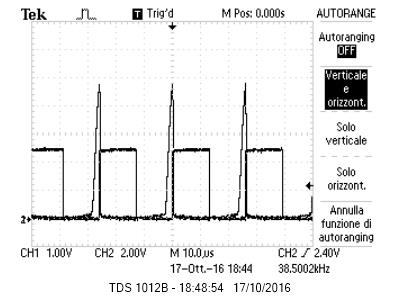
\includegraphics{../oscilloscopio/raise_problem.jpg}
\caption{}
\end{figure}

\end{document}
